
\documentclass[conference]{IEEEtran}

\usepackage{graphicx}
\usepackage{enumerate}
\usepackage[numbers]{natbib}
\usepackage{url} % not crucial - just used below for the URL 
\usepackage{amsmath}
\usepackage{amsfonts}
\usepackage{amssymb}
\usepackage[all]{xy}
\usepackage{color}
\usepackage{subfig}
\usepackage{clrscode}
\usepackage{multirow}
%\usepackage{graphicx,psfrag,epsf}
\newcommand{\fixd}[1]{\textcolor{red}{\bf #1}} %dani's color


% correct bad hyphenation here
\hyphenation{op-tical net-works semi-conduc-tor}


\begin{document}
%
% paper title
% Titles are generally capitalized except for words such as a, an, and, as,
% at, but, by, for, in, nor, of, on, or, the, to and up, which are usually
% not capitalized unless they are the first or last word of the title.
% Linebreaks \\ can be used within to get better formatting as desired.
% Do not put math or special symbols in the title.
\title{Convolutional Neural Networks for Scientific Images: Simulation and Experimental Data}


% author names and affiliations
% use a multiple column layout for up to three different
% affiliations
\author{\IEEEauthorblockN{Michael Shell}
\IEEEauthorblockA{School of Electrical and\\Computer Engineering\\
Georgia Institute of Technology\\
Atlanta, Georgia 30332--0250\\
Email: http://www.michaelshell.org/contact.html}
\and
\IEEEauthorblockN{Homer Simpson}
\IEEEauthorblockA{Twentieth Century Fox\\
Springfield, USA\\
Email: homer@thesimpsons.com}
\and
\IEEEauthorblockN{James Kirk\\ and Montgomery Scott}
\IEEEauthorblockA{Starfleet Academy\\
San Francisco, California 96678--2391\\
Telephone: (800) 555--1212\\
Fax: (888) 555--1212}}


\maketitle

% As a general rule, do not put math, special symbols or citations
% in the abstract
\begin{abstract}
What is the science question we are trying to solve
Why is it hard
Contribution

\end{abstract}

% no keywords


% For peer review papers, you can put extra information on the cover
% page as needed:
% \ifCLASSOPTIONpeerreview
% \begin{center} \bfseries EDICS Category: 3-BBND \end{center}
% \fi
%
% For peerreview papers, this IEEEtran command inserts a page break and
% creates the second title. It will be ignored for other modes.
\IEEEpeerreviewmaketitle

\section{Introduction}
% no \IEEEPARstart
Recent estimates for daily data generation are around 2.5 quintillion ($10^{18}$) bytes. As an example, the instrument upgrades at the Department of Energy (DOE) facilities, including accelerator and signal detector technology, are yielding an unprecedented increase in the quantity and complexity of raw data, especially in multi-domain experimental facilities, such as synchrotrons or neutron sources. The variety of equipment enables thousands of researchers to pursue investigations across a wide range of areas, from archeology and biology to physics and nano-science. While the science is diverse, the underlying image analyses required to measure fundamental quantities about the experiments follow a relatively smaller set of patterns. These patterns or motifs, when incorporated to emerging machine learning (ML) algorithms, will enable scientists to leverage large repositories of curated data, and enable data augmentation as well as discovery at scientifically relevant solution spaces.

Our paper will describe how to turn visual primitives, constrained to space and intensity variations, into higher-level semantics that can be used as computational motifs to understand image-centric data. We include the description and .....
\fixd{here}
 numerical schemes for automated characterization of materials components. Our preliminary use-cases include records of high-resolution data, coming from scientific experiments, particularly those reliant on advanced instruments and simulations. We will address our three main research and development activities:
1) Data sources: by coupling Observational, Simulation, and User-interaction data: how to retrieve
more relevant outcomes, even when using vast amounts of multimodal experimental records;
2) Software tools: we have deployed ML algorithms using deep learning, e.g., convolutional neural
networks for conventional and heterogeneous architectures, such as the low-power consumption IBM True
North neuromorphic chip, as illustrated in Figure 1;
3) Use-cases: we have analyzed large datasets of x-ray scattering data (HipGISAXS), as in Figure 2, running on massively parallel machines, and, more generally, analysis of image-based experiments for quantifying material composition and structures (e.g. QuantCT/IDEAL), exploring graph-based methods. Finally, we will discuss how these images across domains can be processed using similar tools and/or motifs, and how higher levels of concurrency promoted by new computing systems may provide online feedback to steer experiments and collect more information from data.

Use cases in Table~\ref{table1}.

%From joao
The architecture of Convolutional Neural Networks (CNN) depend on a
large number of parameters, obtained from the data and derived weights,
found during a through search over the hyperparameter space. The
memory footprint to compute and store CNN models demand research
on methods to adapt CNN to energy efficient devices. This work focuses
on data reduction schemes and net weight representations in order to
accurately classify scientific data from simulations. Our scheme reduces
double-format values to one byte,maintaining classification accuracy
above 98\%.

%This work incorporates data gathering, analytical schemes using CNN and exploratory visualization.
%Table with all the image modalities discussed in this paper

% Please add the following required packages to your document preamble:
% \usepackage[table,xcdraw]{xcolor}
% If you use beamer only pass "xcolor=table" option, i.e. \documentclass[xcolor=table]{beamer}
\begin{table*}[!]
\centering
\caption{Scientific data under scrutiny with CNN: specifications and methods}
\label{table1}
\begin{tabular}{p{2cm}p{1.6cm}p{1.6cm}p{3cm}p{7.5cm}}
\hline
\rowcolor[HTML]{CCE5FF}
Materials  &  Resolution ($\mu$m)  &  Image \newline modality  &  Imaging  \newline mechanism  &  Data analysis for specimen quantification
\\
\hline
\rowcolor[HTML]{FFFFFF}
material2 \newline whatever & 0.65 to 1.3 & microCT                               & cryo-EM                     & detection something with MatConvNet. Sec.~\ref{subsec:cmc}. Fig.~\ref{fig:microct}.
\\
\hline
\rowcolor[HTML]{F6F6F6}
bragg peaks of what? & 0.65 to 2.5  & diffraction pattern & X-ray diffraction  & detection of Bragg peaks from whatever specimens using MatConvNet. Sec.~\ref{subsec:cmc}. Fig.~\ref{fig:pmrf}.
\\
\hline
\rowcolor[HTML]{FFFFFF}
material2 \newline whatever & 0.65 to 1.3 & microCT  & X-ray attenuation contrast & detection of fiber profile, TensorFlow. Sec.~\ref{subsec:cmc}. Fig.~\ref{fig:microct}.
\\
\hline
\rowcolor[HTML]{F6F6F6}
thin films   & 0.00164  & STEM \newline tomography  & electron transmission    & pore organization across film, associated to level of pore coalescence; surface density analysis correlated to dielectric constant measurements. Sec.~\ref{subsec:stem}. Fig.~\ref{fig:stem}.
\\
\hline
\end{tabular}
\end{table*}


\section{Related work}
Why neuromorphic:
Problem formulation: the most difficult part of computing, neuromorphic or not, is to figure out what to compute, e.g. scale;
Increase data volume, complexity (different imaging conditions, noise levels);
Optimize CNN architecture (number of layer, number of filters, filter size, downsample rate etc.);
Port to TrueNorth (Dharmendra Modha’s blog);
Comparing with other algorithms (e.g., SVM, k-means, kNN, bag of features/signatures):
Complexity and performance;
Flexibility;
Robustness in classification and searchable criterias.
%+bkg
\section{Simulating and recording scientific data}\label{sec:mat}
History about synthesis, screening, characterization, discovery and re-discovery (retrieval)



\begin{figure*}[h!]
\centering
\subfloat[Experimental molecule projections]{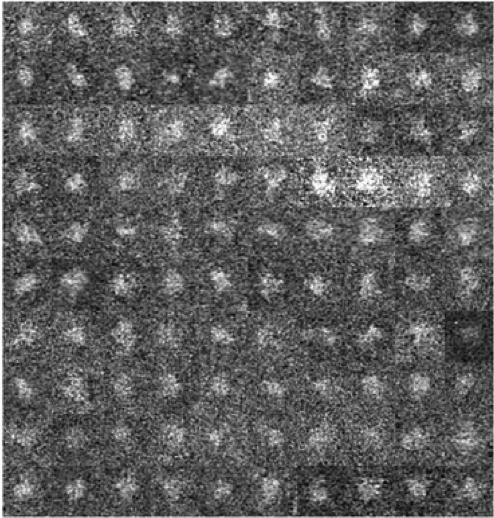
\includegraphics[width=.314\linewidth]{img/cryoem3a.png}
\label{fig_first_case}}
\hfil
\subfloat[Detected particle projections]{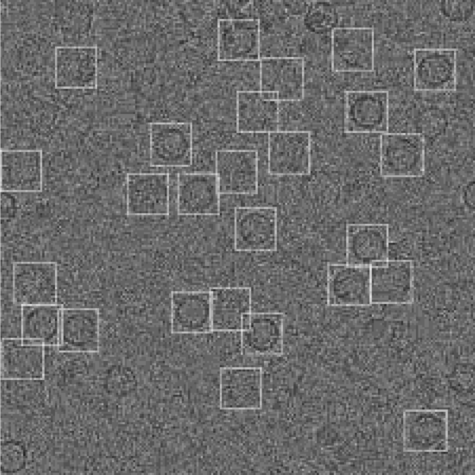
\includegraphics[width=.33\linewidth]{img/cryoem3b.png}
\label{fig_second_case}}
\subfloat[Simulated molecule projections]{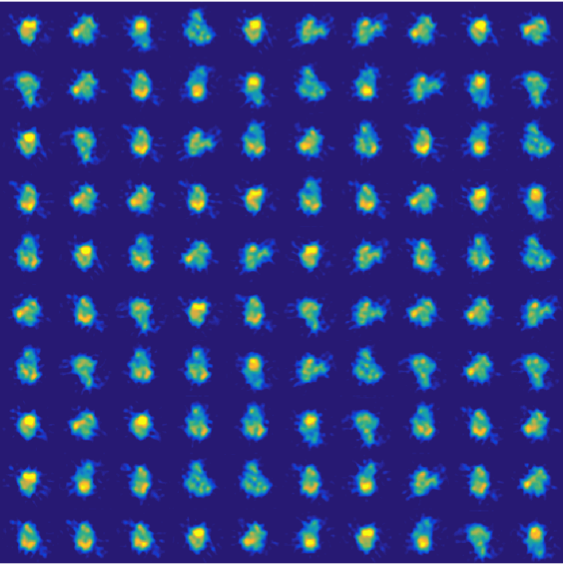
\includegraphics[width=.33\linewidth]{img/cryoem3c.png}
\label{fig_second_case}}
\caption{Cryo-EM images of TFIIDM at different project angles.}
\label{fig:cryo1}
\end{figure*}

%------------------------------------------------------------------------------
%no worries, these marks will be eliminated
-------------------------------------------------------
\subsection{Cryo-EM}\label{subsec:cryo}
Why Cryo-EM?

An important protein is the Transcription initiation factor II because it makes up everything... It has been studied using .... Cryo-EM is a good deal because...

It's hard to get labelled cryo-EM because..., therefore we resort to simulation code to investigate polypeptides. The name of the code and the reference

The data consists of 64 by 64 projection images of TFIID along 9 viewing angles with random perturbation, noise free... What does it have to do with Figure~\ref{fig:cryo1}? What about Figure~\ref{fig:cryo2}?

9 views (evenly spaced on a sphere)
1000 simulated projection images
Projection Euler angles:

chosen randomly from 1 to 9,  generated randomly (uniform distribution) with


\begin{figure*}[th]
\centering
\subfloat[TFIIDM molecule]{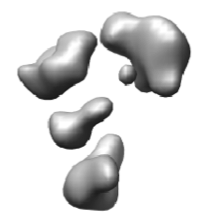
\includegraphics[width=.32\linewidth]{img/cryoem1.png}
\label{fig_first_case}}
\hfil
\subfloat[Projections model]{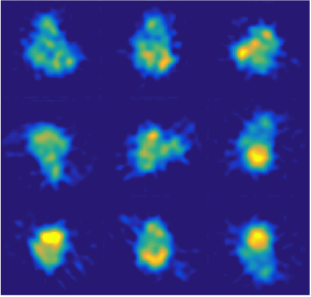
\includegraphics[width=.32\linewidth]{img/cryoem1b.png}
\label{fig_second_case}}
\subfloat[Compact model]{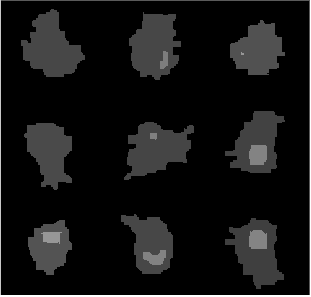
\includegraphics[width=.32\linewidth]{img/cryoem1c.png}
\label{fig_second_case}}
\caption{TFIIDM structure, cryo-EM simulation outcomes and reduced data representation.}
\label{fig:cryo2}
\end{figure*}

%------------------------------------------------------------------------------
%------------------------------------------------------------------------------
-------------------------------------------------------
\subsection{Imaging Techniques based on X-ray}


Synchrotron radiation relies on a charge moving at relativistic speeds, and following a curved trajectory~\cite{url:als:booklet}. The x-ray experimental data used in this article was acquired at the Advanced Light Source, which is a Department of Energy-funded synchrotron facility that provides users from around the world access to the brightest beams of soft x-rays, together with hard x-ray and infrared light, for scientific research and technology development in a wide range of disciplines~\cite{url:als}.

\subsubsection{X-ray diffraction}\label{subsec:diffraction} %LDRD Bragg peaks/Chao
92\% success rate for good images
96\% success rate for bad images
Sufficiently good to distinguish good images from bad images
%92% success rate on images with Bragg peaks
%96% success rate on images with few Bragg peaks

\begin{figure}[!t]
\centering
\subfloat[Hit]{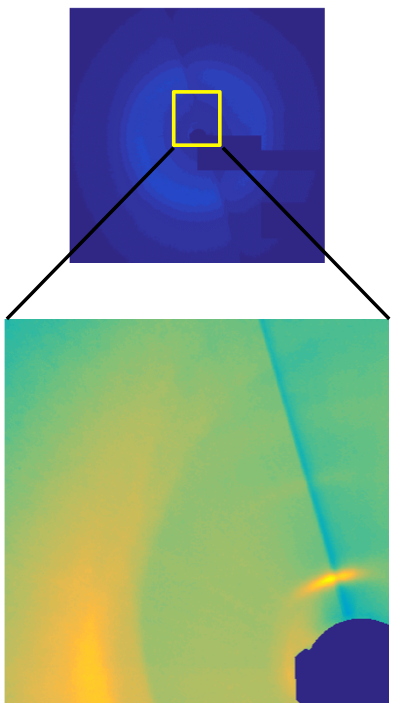
\includegraphics[width=.33\linewidth]{img/bragg1.png}
\label{fig_first_case}}
\hfil
\subfloat[Miss]{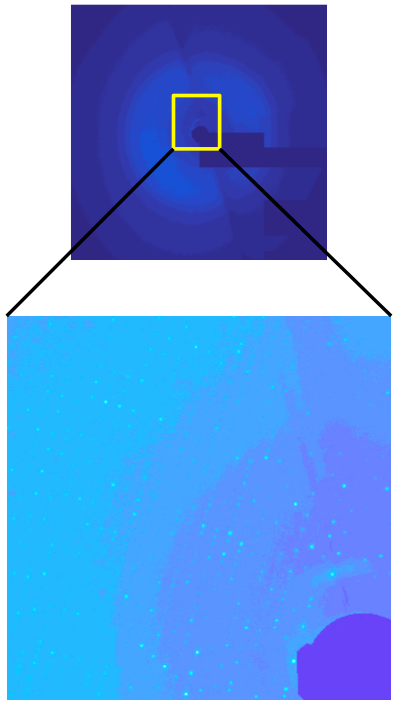
\includegraphics[width=.33\linewidth]{img/bragg2.png}
\label{fig_second_case}}
\caption{LDRD case - bragg peaks.}
\label{fig:ldrd}
\end{figure}

\begin{figure}[!t]
\centering
\subfloat[False negative]{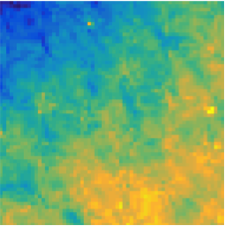
\includegraphics[width=.33\linewidth]{img/xdiffraction_falsenegative.png}
\label{fig_first_case}}
\hfil
\subfloat[False positive]{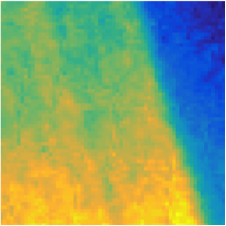
\includegraphics[width=.33\linewidth]{img/xdiffraction_falsepositive.png}
\label{fig_second_case}}
\caption{LDRD case - bragg peaks.}
\label{fig:ldrd}
\end{figure}

%------------------------------------------------------------------------------
-------------------------------------------------------
\subsubsection{X-ray scattering}\label{subsec:gisaxs} %Alex
Scattering techniques are very well established and used to probe micro and nano-structures with a high degree of statistical relevance. The most prominent techniques are small angle X-ray and neutron scattering (SAXS and SANS) for the detection of mesoscale structures as well as wide angle X-ray and neutron scattering (WAXS and WANS) for the investigation of the structure down to the molecular scale. Prominent examples are thin films of conductive polymers, organic electronics, or thin films of nano-particles, which receive high interest for energy relevant materials such as organic photovoltaics. Morphological characterization of thin films is challenging, and substantial advancements have been accomplished through research efforts on new experimental geometry setups for scattering. Unfortunately, these have not been enough to provide the required data reduction and analysis that is fundamental for giving scientist access to use advanced grazing incidence techniques and getting the most relevant information out of their experiments. In particular in-situ analysis is far from possible at the given time.

We propose a supervised classification approach to identify the crystal lattice types from a Grazing Incidence Small Angle X-ray Scattering (GISAXS) image. GISAXS is an important reciprocal-space imaging modality which provides statistical information about a sample in 3-D. GISAXS is widely used for
studying thin films that play a vital role as building blocks for the next generation of renewable energy technology. One challenge in GISAXS imaging is to accurately infer the crystal lattice corresponding to the sample from a single 2-D diffraction/scatter pattern.

\begin{figure}[!t]
\centering
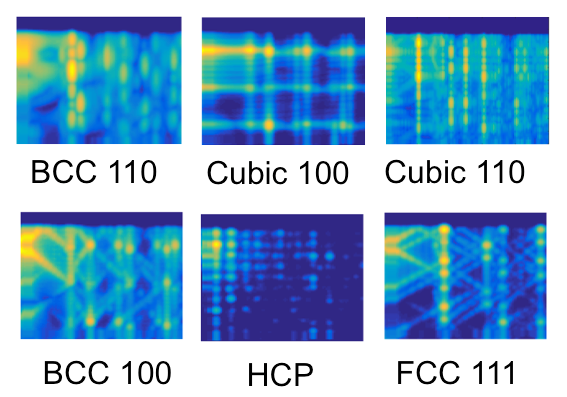
\includegraphics[width=.439\linewidth]{img/gisaxs1.png}
\caption{Figure to be replaced by Venkat.}
\label{fig:gisaxs}
\end{figure}

As a first step towards understanding crystal configurations, we use a simulation package termed HiPGISAXS [1], to generate a large collection of sample images from each class of possible crystal structures and test the algorithm performance under multiple simulated test images. Inspired by the
recent successes of deep-learning approaches for natural image classification, we tested CNN as the method to carry out the classification.

We have been exploring detection of peak-positions from image datasets, so that information about the lattice and orientation of the material is recovered. A typical image from the ALS beamline 7.3.3 will present shapes used as input to derive the underlying structure of the sample. The location, shapes and position of these structures, while yielding useful information, can also be used as an input to simulation tools. Shapes vary among rings, arcs, peaks and lines. In case of time resolved or multi-energy data, the features become three or more dimensional, e.g., peaks become rods and lines become planes. We will develop software tools for the pattern recognition of the scattering data collected in grazing incidence geometry. The task of extracting morphological structures and representing them through features maps will have similarities to pattern recognition in 3D tomography data. Advanced recognition will significantly accelerate the model development for forward solvers.

%------------------------------------------------------------------------------
-------------------------------------------------------
\subsubsection{X-ray attenuation contrast}\label{subsec:microct}
Another example of high-throughput data collection is microct....


the study of ceramic matrix composites, which are hierarchical materials, composed of many individual strands, bundled within a matrix, after which bundles are woven together. To simulate the operating conditions for which these materials are designed, they are heated to nearly 2,000 degrees and then stressed, causing both cracks in the matrix and the breaking of individual fibers. In both of the cases mentioned above, currently the researchers collect a series of 3D images as a function of time. After the experiment, the researchers often go through the 3D images manually, slice by slice, looking for the individual dendrites or “delaminations” that form in the batteries which correlate with decreased performance, or for the broken fibers or matrix cracks. This is a very time-consuming process.

Proposed work and expected solutions: Develop and deploy algorithms that find these features using raw microCT images as input, and then point out which of the experimental instances (image stacks) present the structures of interest. Being able to detect these features in real time will add an entirely new level of experimental capability. Tying this capability in with the control systems at the beamline will allow the experiment to be controlled by the machine in response to which structures the sample presents. For example, when a feature of interest is found, the process may be temporarily slowed down while a magnified image is collected of the region of interest, before resuming the process. Currently, it is unlikely that the users will find detailed features of interest in their images fast enough to be able to adjust the parameters of their experiment to collect optimal data. By having recognition closer to the detector, we will be able to obtain higher resolution data in specific regions, or more time points during a transition of interest.


\cite{IEEEBigData:2014}


\begin{figure}[!t]
\centering
\subfloat[Case I]{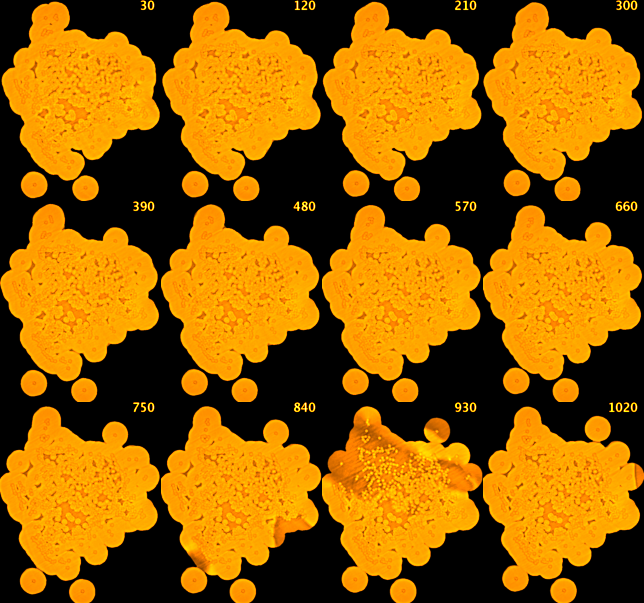
\includegraphics[width=.439\linewidth]{img/fiberMontage.png}
\label{fig_first_case}}
%\hfil
\subfloat[Case II]{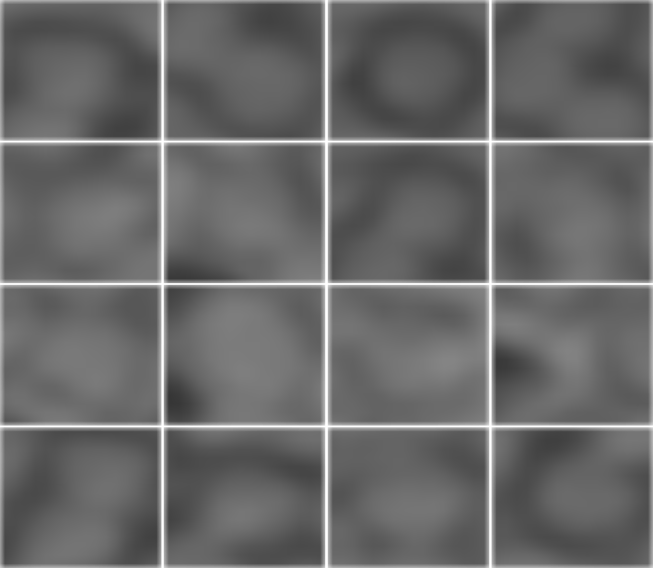
\includegraphics[width=.475\linewidth]{img/yes_fibers.png}
\label{fig_second_case}}
\caption{Some description of CMC and fibers.}
\label{fig:microct}
\end{figure}

\section{Convolutional neural networks}
Synapses enable nerve cells to connect to thousands of other neurons, combine signals, and push the integrated information forward. Early research by Hubel and Wiesel [1] on the cat’s visual cortex showed that neurons propagate information through complex cell organizations called receptive fields [2]. These fields work similarly to filters for the stimuli coming from previous retinal layers, and allow information from 125 million photoreceptors to be successfully processed and pushed forward to 1 million ganglion cells along the visual processing path. These biological filters can be framed in an algorithmic motif that exploits the strong spatially local correlation present in digital images in learning tasks. As an example of such algorithms, convolutional neural networks (CNNs) have been successfully used in pattern recognition because CNN can learn a hierarchy of features by building high-level features from low-level ones, thereby automating the process of feature construction [3, 4], much differently from traditional approaches.

In this section, we introduce the proposed Convolutional Neural Networks algorithms used for scientific image exploration and understanding under four modalities
, which consists of three main

why different science problems are being attached by different algorithms? Are there differences in the architecture of these different algorithms?

On the convergence of classification algorithms for

\subsection{Matconvnet}

\subsubsection{Neuromophic computation}


\subsection{TensorFlow}

\section{Results}
In order to improve understanding of our experimental results, we keep the subsections organized per use-cases, as described in Sec.~\ref{sec:mat}.

\subsection{Cryo-EM and molecule projections}
A traditional Convolutional Neural Network (CNN) is parameterized by floating point weights and biases and takes floating point data as input. In many cases, the floating point representation of these parameters and input is more than necessary. The use of a more compact representation of the parameters and input allows CNNs to be deployed on energy efficient architectures that operate with a few bits and much lower memory footprint. This work focuses on data reduction and quantization schemes that can be applied to a trained CNN for classifying scienti c simulation data. We show that each
neuron and synapse can be encoded with only one byte to maintain accuracy above 98\%.

\begin{figure}[h]
\centering
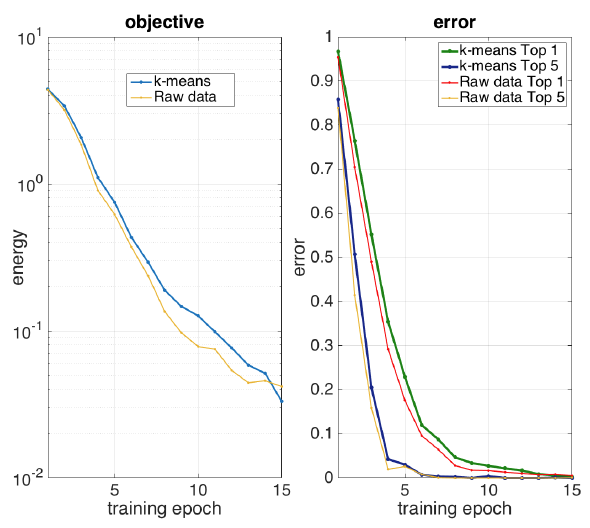
\includegraphics[width=\linewidth]{img/joao3.png}
\caption{Simulation results for the network.}
\label{fig_sim}
\end{figure}


64 by 64 projection images of TFIID along 9 viewing angles with random perturbation, noise free;

\begin{table}[]
\centering
\caption{Parameters for the simulation models of TFIID projects.}
\label{my-label}
\begin{tabular}{|c|c|c|}
\hline
 $\Psi\downarrow_i$    & $\Theta\downarrow_i$       & $\phi\downarrow_i$
 \\
 \hline
0.00 & 0.0000 & 0.0000 \\
0.00 & 45.000 & 0.0000 \\
0.00 & 45.000 & 89.975 \\
0.00 & 45.000 & 179.95 \\
0.00 & 45.000 & 269.92 \\
0.00 & 90.000 & 0.0000 \\
0.00 & 90.000 & 59.983 \\
0.00 & 90.000 & 119.97 \\
0.00 & 90.000 & 178.95 \\
\hline
\end{tabular}
\end{table}

\textbf{Classifying 9 views:}
Training images generated from a 3D density map of a transcription factor-II

\textbf{Testing}
100 projection images generated from Euler angles
 chosen randomly from 1 to 9
,  generated randomly (uniform distribution) with
Result: 100\% success rate

\subsection{Imaging Techniques based on X-ray}
\subsubsection{X-ray diffraction}

\subsubsection{X-ray scattering}
We address the problem of classifying GISAXS patterns from 7 different crystal lattices (classes). We generated 1,000 images with dimensions of 100X100 pixels for each class by varying the lattice parameters as input to a 4 layer CNN to train a classifier. The architecture of this network is adapted from the MNIST classifier used by MatConvNet. We tested the performance of the classifier on
multiple data sets, including samples corrupted with realistic noise levels. We obtained an accuracy that ranged from 82.6\% to 92.29\% depending on the parameters of each test case which we believe is an encouraging result for further extending the use of CNNs for GISAXS as well as other synchrotron based scientific experiments.

\begin{table}[]
\centering
\caption{My caption}
\label{my-label}
\begin{tabular}{|c||c|c|c|}
\hline
Method & dataset1 & dataset2 & noisyDataset \\
\hline
CNN    & 92.29    & 82.60    & 91.57        \\
HOG    & 92.00    & 79.88    & 79.57        \\
\hline
\end{tabular}
\end{table}

\begin{table}[]
\centering
\caption{My caption}
\label{my-label}
\begin{tabular}{|c||c|c|c|}
\hline
Method & dataset1 & dataset2 & noisyDataset \\
\hline
CNN    & 92.29    & 82.60    & 91.57        \\
HOG    & 92.00    & 79.88    & 79.57        \\
\hline
\end{tabular}
\end{table}

\subsubsection{X-ray attenuation contrast}

\textbf{Neuromorphic computing}
- Eedn
- Corelet Laboratory: Corelet Language + Corelet Library (used to configure the neural network)
COMPASS simulator
Available for IBM Blue Gene Q;
Average neuron spiking rate 8.1 Hz (388 times slower than real time);
Support both MPI and OpenMP and PGAS;

The job of a TrueNorth programmer is to translate a desired computation into a specified network of neurosynaptic cores, its inputs and outputs through corelets
In this project, we will produce corelets for several image analysis and pattern recognition problems relevant to DOE science applications

Challenges: Can we build a computer that works like a brain?
Quick classification, pattern recognition
Low power
Fault tolerant
Easy to program


%\begin{figure}[h]
%\centering
%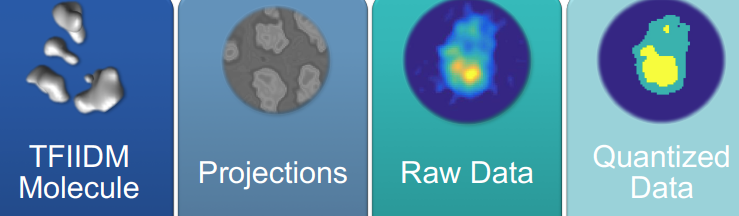
\includegraphics[width=\linewidth]{img/joao1.png}
%\caption{Simulation results for the network.}
%\label{fig_sim}
%\end{figure}

\begin{figure}[h]
\centering
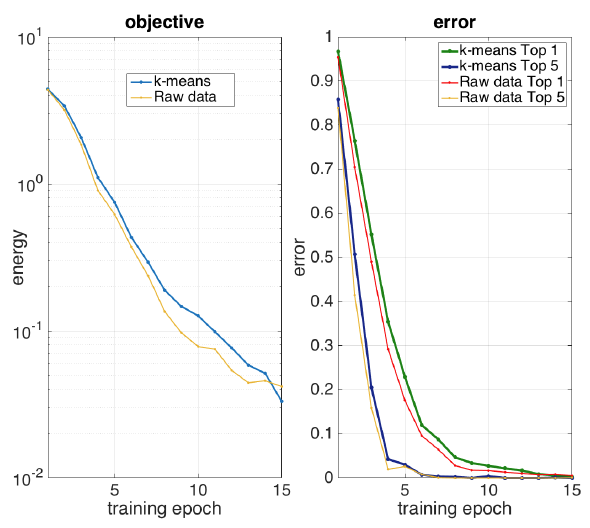
\includegraphics[width=\linewidth]{img/joao3.png}
\caption{Coisas do jao.}
\label{fig:cryem}
\end{figure}

IBM TN settings:
Corelet Programming Environment CPE Version 2.2.160518
CPE + tn-signal-processor to make a model
and run a model on the TrueNorth hardware
Matlab with MatConvNet

Fibers=216,650 samples
Non-fibers=105,120 samples
Each sample = 162 uint8 input (raw = no processing)
How: leverage curated data analyzed using sophisticated computer vision algorithms + user intervention

Preliminary results using the neuromorphic chip IBM TrueNorth
Specs and accuracy:
~3,200 cores < 1 chip = 4096 cores
Model =
Train=70\%; test=30\%
Accuracy = 99.788623\%

What is next:
Interpret Eedn output results
Deploy TN on a testbed at NERSC
Port models to the chip at LBL
Evaluate on new samples coming from ALS

\subsection{NVIDIA DevBox}

pyCBIR is python package that offers a prototype system for user exploration of general image composition. The system enables image-based query to digital imagery archives, returning the top-n pictures that most resembles the query.


%Our search engine builds upon computer vision advances made over the past decade in low-level feature matching, large data handling and object recognition. We demonstrate hierarchical clustering among images semi-cooperatively shot around MIT, automatic linking of flickr photos and aerial frames from the Grand Canyon, and video segment identification for a TV broadcast. Moreover, our software tools incorporate visible vs infrared band selection, color content quantization and human face detection. Ongoing and future extensions of this image search system are discussed.


\begin{figure}[!t]
\centering
\subfloat[Case I]{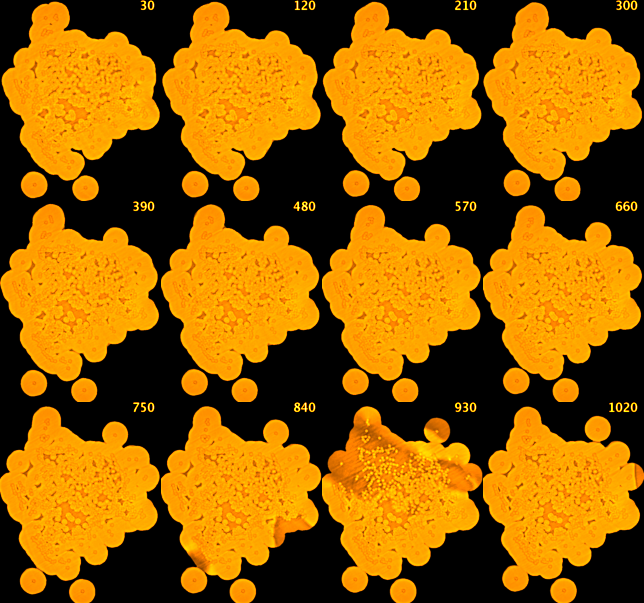
\includegraphics[width=.439\linewidth]{img/fiberMontage.png}
\label{fig_first_case} \\ }
%\hfil
\subfloat[Case II]{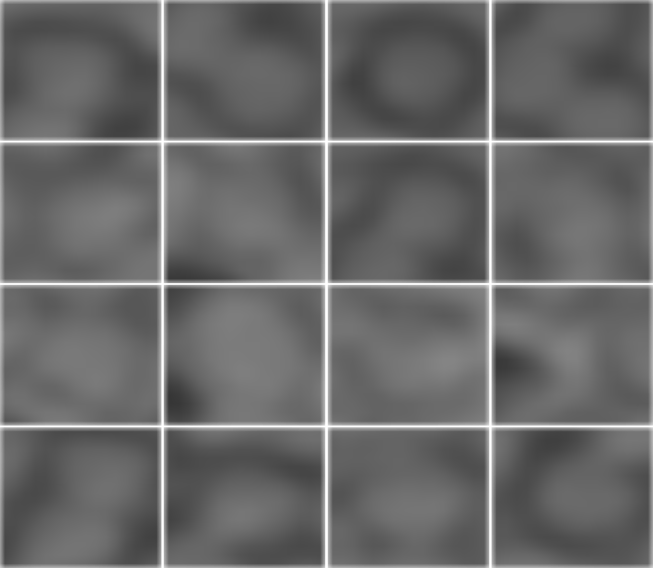
\includegraphics[width=.475\linewidth]{img/yes_fibers.png}
\label{fig_second_case}}
\caption{Using TensorFlow: Dataset with more than three hundred thousand samples, used to train a deep
learning algorithm in order to separate fiber profiles (left) from other regions (right) as they
appear in micro tomography image from ceramic matrix composites. Accuracy results for this CNN are
99.788623\%, considering stratified training and tests sets, with 70\% and 30\% of the samples
respectively.}
\label{fig:pycbir}
\end{figure}



% \begin{table}[!h]
% \caption{This is only a place holder for table.}\label{tab:accTari} \centering
% \begin{tabular}{|c||c|c|c|}
%   \hline
%   \multirow{2}{*}{\textbf{Method}} & \textbf{Tari 56} & \textbf{Tari 180} & \textbf{Tari 1000} \\
%    & \textbf{Database} & \textbf{Database} & \textbf{Database} \\
%   \hline
%   Proposed & \textbf{99.84\%} & \textbf{96.66\%} & \textbf{81.60\%} \\
%   \hline
%   ProposedNoConc & 93.82\% & 90.84\% & 73.96\% \\
%   \hline
%   PedrosaA \cite{Pedrosa:2011a} & 43.25\% & 26.40\% & 15.49\% \\
%   \hline
%   PedrosaB \cite{Pedrosa:2011b} & 75.06\% & 61.46\% & 53.35\% \\
%   \hline
%   PedrosaBConc & \textbf{76.48\%} & \textbf{66.13\%} & \textbf{57.83\%} \\
%   \hline
%   TAR & 86.30\% & 84.86\% & 64.27\% \\
%   \hline
% \end{tabular}
% \end{table}


\section{Conclusion}
The conclusion goes here.
%+disc
% use section* for acknowledgment
\section{Future developments}
\section*{Acknowledgment}


The authors would like to thank...
 %+ack

\section{Introduction}
% no \IEEEPARstart
Recent estimates for daily data generation are around 2.5 quintillion ($10^{18}$) bytes. As an example, the instrument upgrades at the Department of Energy (DOE) facilities, including accelerator and detector technology, are yielding an unprecedented increase in the quantity and complexity of raw data, especially in multi-domain experimental facilities, such as synchrotrons or neutron sources. The variety of equipment enables thousands of researchers to pursue investigations across a wide range of areas, from archeology and biology to physics and nano-science. While the science is diverse, the underlying image analyses required to measure fundamental quantities about the experiments, follow a
relatively smaller set of patterns. These patterns or motifs consist of statistical schemes and data formats, which when incorporated to emerging machine learning (ML) algorithms, can leverage large repositories of curated data, and enable discovery at scientifically relevant solution spaces.

Our paper will describe how space and intensity variations work as computational motifs and how to use ML algorithms to image-centric data, including numerical schemes for automated characterization of materials components. Our preliminary use-cases include records of high-resolution data, coming from scientific experiments, particularly those reliant on advanced instruments and simulations. We will address our three main research and development activities:
1) Data sources: by coupling Observational, Simulation, and User-interaction data: how to retrieve
more relevant outcomes, even when using vast amounts of multimodal experimental records;
2) Software tools: we have deployed ML algorithms using deep learning, e.g., convolutional neural
networks for conventional and heterogeneous architectures, such as the low-power consumption IBM True
North neuromorphic chip, as illustrated in Figure 1;
3) Use-cases: we have analyzed large datasets of x-ray scattering data (HipGISAXS), as in Figure 2,
running on massively parallel machines, and, more generally, analysis of image-based experiments for
quantifying material composition and structures (e.g. QuantCT/IDEAL), exploring graph-based methods.
Finally, we will discuss how these images across domains can be processed using similar tools and/or
motifs, and how higher levels of concurrency promoted by new computing systems may provide online
feedback to steer experiments and collect more information from data.


%From joao
The architecture of Convolutional Neural Networks (CNN) depend on a
large number of parameters, obtained from the data and derived weights,
found during a through search over the hyperparameter space. The
memory footprint to compute and store CNN models demand research
on methods to adapt CNN to energy efficient devices. This work focuses
on data reduction schemes and net weight representations in order to
accurately classify scientific data from simulations. Our scheme reduces
double-format values to one byte,maintaining classification accuracy
above 98\%.



\section{Related work}
Why neuromorphic:
Problem formulation: the most difficult part of computing, neuromorphic or not, is to figure out what to compute, e.g. scale;
Increase data volume, complexity (different imaging conditions, noise levels);
Optimize CNN architecture (number of layer, number of filters, filter size, downsample rate etc.);
Port to TrueNorth (Dharmendra Modha’s blog);
Comparing with other algorithms (e.g., SVM, k-means, kNN, bag of features/signatures):
Complexity and performance;
Flexibility;
Robustness in classification and searchable criterias.


\section{Simulating and recording scientific data}
History about synthesis, screening, characterization, discovery and re-discovery (retrieval)

\subsection{Cryo-EM}
chao/joao
64 by 64 projection images of TFIID along 9 viewing angles with random perturbation, noise free);

\begin{table}[]
\centering
\caption{My caption}
\label{my-label}
\begin{tabular}{|c|c|c|}
 $\Psi\downarrow_i$    & $\Theta\downarrow_i$       & $\phi\downarrow_i$       \\
0.00 & 0.0000 & 0.0000 \\
0.00 & 45.000 & 0.0000 \\
0.00 & 45.000 & 89.975 \\
0.00 & 45.000 & 179.95 \\
0.00 & 45.000 & 269.92 \\
0.00 & 90.000 & 0.0000 \\
0.00 & 90.000 & 59.983 \\
0.00 & 90.000 & 119.97 \\
0.00 & 90.000 & 178.95
\end{tabular}
\end{table}

\textbf{Classifying 9 views:}
Training images generated from a 3D density map of a transcription factor-II

\textbf{Testing}
100 projection images generated from Euler angles 
 chosen randomly from 1 to 9 
,  generated randomly (uniform distribution) with 
Result: 100\% success rate





9 views (evenly spaced on a sphere)
1000 simulated projection images
Projection Euler angles:

 chosen randomly from 1 to 9
,  generated randomly (uniform distribution) with 

\begin{figure*}[!t]
\centering
\subfloat[Experimental molecule projections]{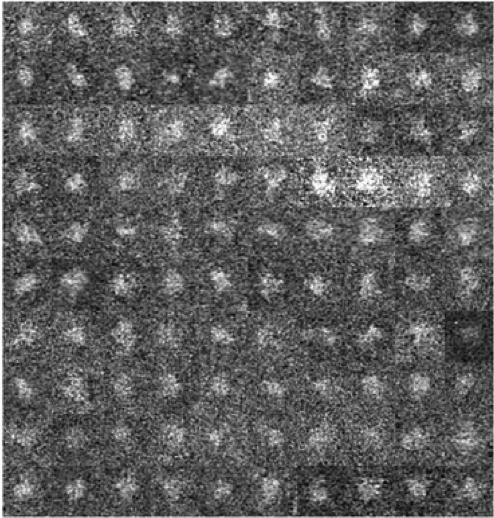
\includegraphics[width=.314\linewidth]{img/cryoem3a.png}
\label{fig_first_case}}
\hfil
\subfloat[Detected particle projections]{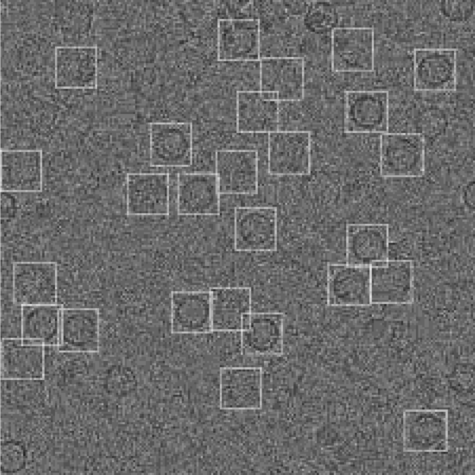
\includegraphics[width=.33\linewidth]{img/cryoem3b.png}
\label{fig_second_case}}
\subfloat[Simulated molecule projections]{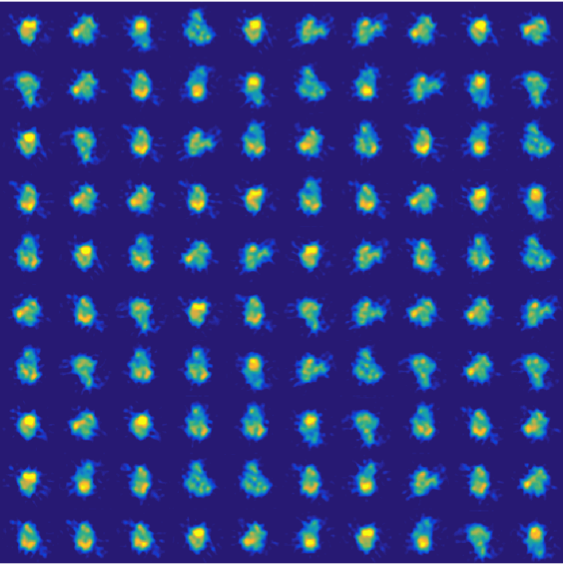
\includegraphics[width=.33\linewidth]{img/cryoem3c.png}
\label{fig_second_case}}
\caption{LDRD case.}
\label{fig:ldrd}
\end{figure*}

\begin{figure*}[!t]
\centering
\subfloat[TFIIDM molecule]{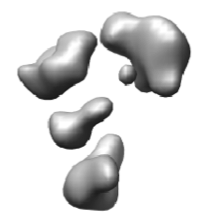
\includegraphics[width=.32\linewidth]{img/cryoem1.png}
\label{fig_first_case}}
\hfil
\subfloat[Projections model]{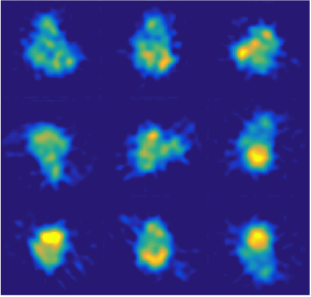
\includegraphics[width=.32\linewidth]{img/cryoem1b.png}
\label{fig_second_case}}
\subfloat[Compact model]{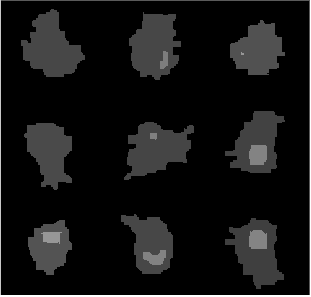
\includegraphics[width=.32\linewidth]{img/cryoem1c.png}
\label{fig_second_case}}
\caption{LDRD case.}
\label{fig:ldrd}
\end{figure*}



\subsection{X-ray diffraction} %LDRD Bragg peaks
92\% success rate for good images
96\% success rate for bad images
Sufficiently good to distinguish good images from bad images
%92% success rate on images with Bragg peaks
%96% success rate on images with few Bragg peaks

\begin{figure}[!t]
\centering
\subfloat[Hit]{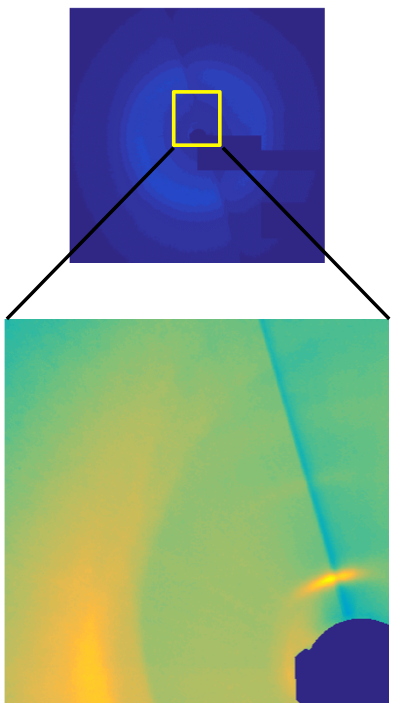
\includegraphics[width=.33\linewidth]{img/bragg1.png}
\label{fig_first_case}}
\hfil
\subfloat[Miss]{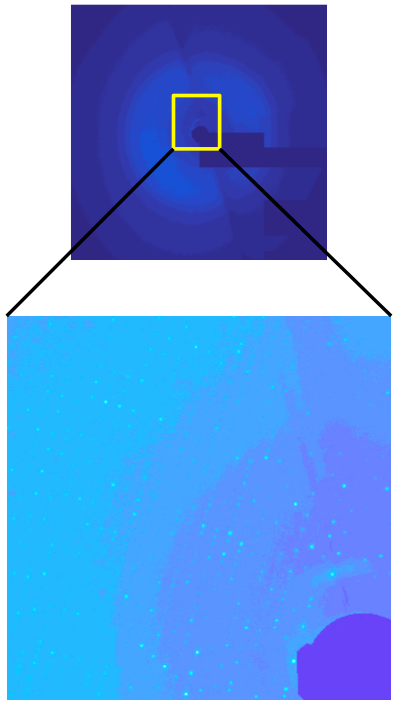
\includegraphics[width=.33\linewidth]{img/bragg2.png}
\label{fig_second_case}}
\caption{LDRD case - bragg peaks.}
\label{fig:ldrd}
\end{figure}

\begin{figure}[!t]
\centering
\subfloat[False negative]{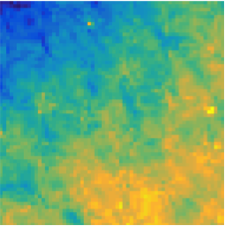
\includegraphics[width=.33\linewidth]{img/xdiffraction_falsenegative.png}
\label{fig_first_case}}
\hfil
\subfloat[False positive]{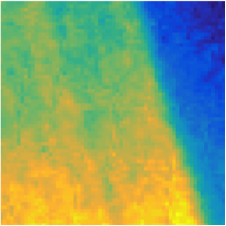
\includegraphics[width=.33\linewidth]{img/xdiffraction_falsepositive.png}
\label{fig_second_case}}
\caption{LDRD case - bragg peaks.}
\label{fig:ldrd}
\end{figure}




\subsection{Scattering}
We propose a supervised classification approach to identify the crystal lattice types from a Grazing
Incidence Small Angle X-ray Scattering (GISAXS) image. GISAXS is an important reciprocal-space imaging
modality which provides statistical information about a sample in 3-D. GISAXS is widely used for
studying thin films that play a vital role as building blocks for the next generation of renewable
energy technology. One challenge in GISAXS imaging is to accurately infer the crystal lattice
corresponding to the sample from a single 2-D diffraction/scatter pattern.

As a first step towards understanding crystal configurations, we use a simulation package termed
HiPGISAXS [1], to generate a large collection of sample images from each class of possible crystal
structures and test the algorithm performance under multiple simulated test images. Inspired by the
recent success of deep-learning approaches for natural image classification, we use a Convolutional
Neural Network (CNN) [2] method to carry out the classification.

We address the problem of classifying GISAXS patterns from 7 different crystal lattices (classes). We
generated 1,000 images with dimensions of 100X100 pixels for each class by varying the lattice
parameters as input to a 4 layer CNN to train a classifier. The architecture of this network is
adapted from the MNIST classifier used by MatConvNet. We tested the performance of the classifier on
multiple data sets, including samples corrupted with realistic noise levels. We obtained an accuracy
that ranged from 82.6\% to 92.29\% depending on the parameters of each test case which we believe is
an encouraging result for further extending the use of CNNs for GISAXS as well as other synchrotron
based scientific experiments.

\begin{table}[]
\centering
\caption{My caption}
\label{my-label}
\begin{tabular}{llll}
Method & dataset1 & dataset2 & noisyDataset \\
CNN    & 92.29    & 82.60    & 91.57        \\
HOG    & 92.00    & 79.88    & 79.57        \\
       &          &          &             
\end{tabular}
\end{table}

\subsection{Phase contrast}



%

\section{Results}

\subsection{Matconvnet}
A traditional Convolutional Neural Network (CNN) is parameterized by floating point weights and biases
and takes floating point data as input. In many cases, the floating point representation of these
parameters and input is more than necessary. The use of a more compact representation of the
parameters and input allows CNNs to be deployed on energy efficient architectures that operate with a
few bits and much lower memory footprint. This work focuses on data reduction and quantization schemes
that can be applied to a trained CNN for classifying scienti c simulation data. We show that each
neuron and synapse can be encoded with only one byte to maintain accuracy above 98\%.
\begin{figure}[h]
\centering
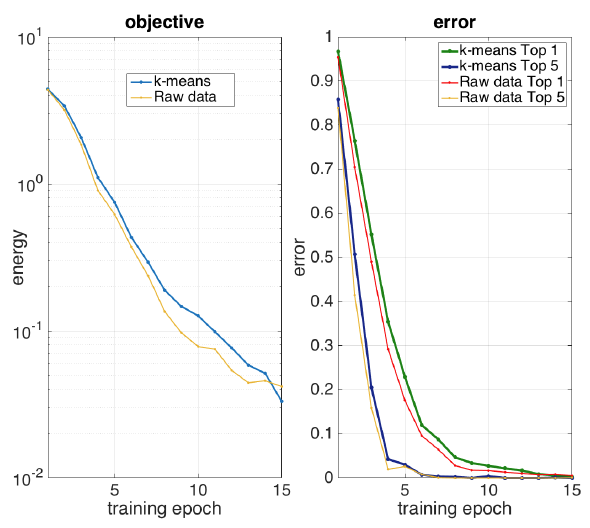
\includegraphics[width=\linewidth]{img/joao3.png}
\caption{Simulation results for the network.}
\label{fig_sim}
\end{figure}


\subsection{Neuromorphic computing}
Corelet Laboratory: Corelet Language + Corelet Library (used to configure the neural network)
COMPASS simulator
Available for IBM Blue Gene Q;
Average neuron spiking rate 8.1 Hz (388 times slower than real time);
Support both MPI and OpenMP and PGAS;

The job of a TrueNorth programmer is to translate a desired computation into a specified network of neurosynaptic cores, its inputs and outputs through corelets
In this project, we will produce corelets for several image analysis and pattern recognition problems relevant to DOE science applications

Challenges: Can we build a computer that works like a brain?
Quick classification, pattern recognition
Low power
Fault tolerant
Easy to program


%\begin{figure}[h]
%\centering
%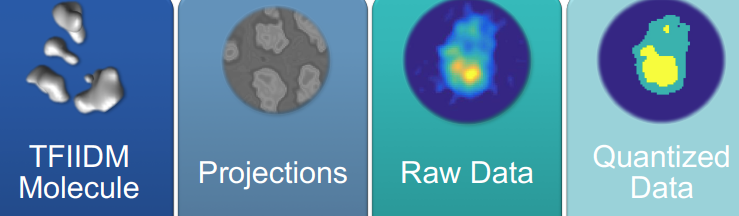
\includegraphics[width=\linewidth]{img/joao1.png}
%\caption{Simulation results for the network.}
%\label{fig_sim}
%\end{figure}

\begin{figure}[h]
\centering
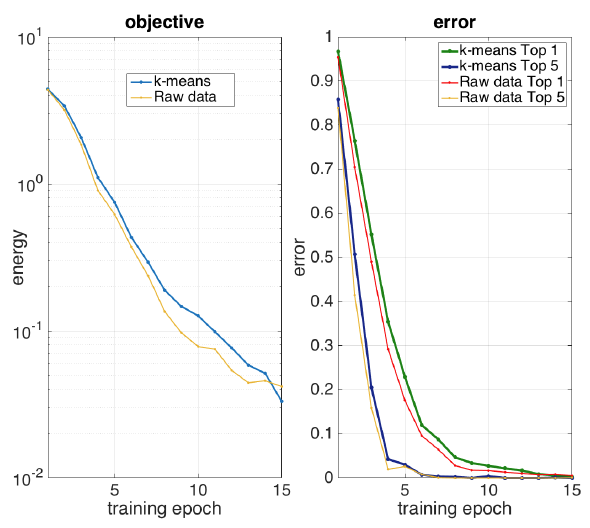
\includegraphics[width=\linewidth]{img/joao3.png}
\caption{Coisas do jao.}
\label{fig:cryem}
\end{figure}

IBM TN settings:
Corelet Programming Environment CPE Version 2.2.160518
CPE + tn-signal-processor to make a model
and run a model on the TrueNorth hardware
Matlab with MatConvNet

Fibers=216,650 samples
Non-fibers=105,120 samples
Each sample = 162 uint8 input (raw = no processing)
How: leverage curated data analyzed using sophisticated computer vision algorithms + user intervention

Preliminary results using the neuromorphic chip IBM TrueNorth
Specs and accuracy:
~3,200 cores < 1 chip = 4096 cores
Model = 
Train=70\%; test=30\%
Accuracy = 99.788623\%

What is next:
Interpret Eedn output results
Deploy TN on a testbed at NERSC
Port models to the chip at LBL
Evaluate on new samples coming from ALS

\subsection{NVIDIA DevBox}



\begin{figure*}[!t]
\centering
\subfloat[Case I]{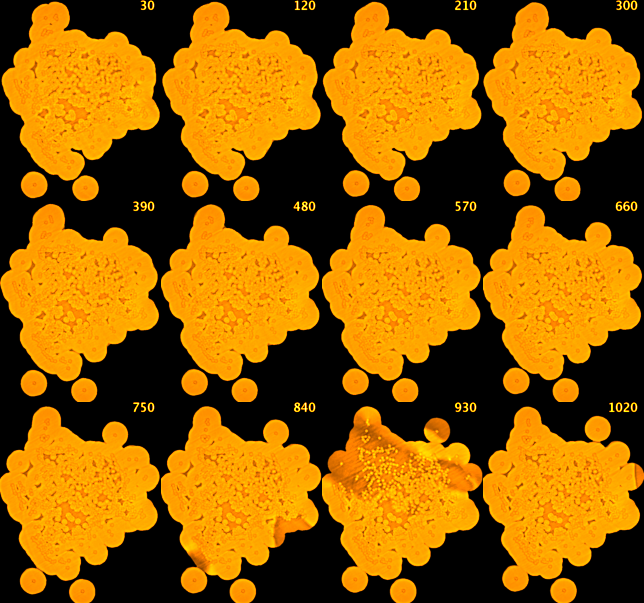
\includegraphics[width=.439\linewidth]{img/fiberMontage.png}
\label{fig_first_case}}
\hfil
\subfloat[Case II]{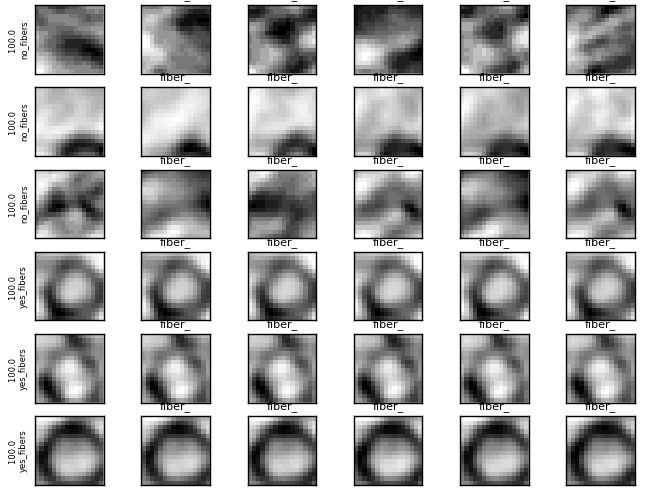
\includegraphics[width=.54\linewidth]{img/fiberCBIR.png}
\label{fig_second_case}}
\caption{Using TensorFlow: Dataset with more than three hundred thousand samples, used to train a deep
learning algorithm in order to separate fiber profiles (left) from other regions (right) as they
appear in micro tomography image from ceramic matrix composites. Accuracy results for this CNN are
99.788623\%, considering stratified training and tests sets, with 70\% and 30\% of the samples
respectively.}
\label{fig:pycbir}
\end{figure*}

\begin{table}[!h]
\caption{This is only a place holder for table.}\label{tab:accTari} \centering
\begin{tabular}{|c||c|c|c|}
  \hline
  \multirow{2}{*}{\textbf{Method}} & \textbf{Tari 56} & \textbf{Tari 180} & \textbf{Tari 1000} \\
   & \textbf{Database} & \textbf{Database} & \textbf{Database} \\
  \hline
  Proposed & \textbf{99.84\%} & \textbf{96.66\%} & \textbf{81.60\%} \\
  \hline
  ProposedNoConc & 93.82\% & 90.84\% & 73.96\% \\
  \hline
  PedrosaA \cite{Pedrosa:2011a} & 43.25\% & 26.40\% & 15.49\% \\
  \hline
  PedrosaB \cite{Pedrosa:2011b} & 75.06\% & 61.46\% & 53.35\% \\
  \hline
  PedrosaBConc & \textbf{76.48\%} & \textbf{66.13\%} & \textbf{57.83\%} \\
  \hline
  TAR & 86.30\% & 84.86\% & 64.27\% \\
  \hline
\end{tabular}
\end{table}


\section{Conclusion}
The conclusion goes here.




% conference papers do not normally have an appendix


% use section* for acknowledgment
\section*{Acknowledgment}


The authors would like to thank...





% trigger a \newpage just before the given reference
% number - used to balance the columns on the last page
% adjust value as needed - may need to be readjusted if
% the document is modified later 
%\IEEEtriggeratref{8}
% The "triggered" command can be changed if desired:
%\IEEEtriggercmd{\enlargethispage{-5in}}

% references section

% can use a bibliography generated by BibTeX as a .bbl file
% BibTeX documentation can be easily obtained at:
% http://mirror.ctan.org/biblio/bibtex/contrib/doc/
% The IEEEtran BibTeX style support page is at:
% http://www.michaelshell.org/tex/ieeetran/bibtex/
%\bibliographystyle{IEEEtran}
% argument is your BibTeX string definitions and bibliography database(s)
%\bibliography{IEEEabrv,../bib/paper}
%
% <OR> manually copy in the resultant .bbl file
% set second argument of \begin to the number of references
% (used to reserve space for the reference number labels box)
\begin{thebibliography}{1}

\bibitem{IEEEhowto:kopka}
H.~Kopka and P.~W. Daly, \emph{A Guide to \LaTeX}, 3rd~ed.\hskip 1em plus
  0.5em minus 0.4em\relax Harlow, England: Addison-Wesley, 1999.

\end{thebibliography}




% that's all folks
\end{document}


